%% if you are submitting an initial manuscript then you should have submission as an option here
%% if you are submitting a revised manuscript then you should have revision as an option here
%% otherwise options taken by the article class will be accepted
\documentclass[submission]{FPSAC2022}
%% but DO NOT pass any options (or change anything else anywhere) which alters page size / layout / font size etc

%% note that the class file already loads {amsmath, amsthm, amssymb}

\newtheorem{thm}{Theorem}
\newtheorem{lem}{Lemma}

\usepackage{lipsum}

%% define your title in the usual way
\title[Optional shorter title]{Something to do with math}

%% define your authors in the usual way
%% use \addressmark{1}, \addressmark{2} etc for the institutions, and use \thanks{} for contact details
\author[Optional shorter names]{Longer names me\thanks{\href{mailto:hello@world.c}{hello@world.c}. Longer names me was partially supported by Grant 2017.11.14.$\partial$\;supp.}\addressmark{1}, \and you\addressmark{2}}

%% then use \addressmark to match authors to institutions here
\address{\addressmark{1}Department of This, University of That, There \\ \addressmark{2}School of Something, University of Something Else, Somewhere}

%% put the date of submission here
\received{\today}

%% leave this blank until submitting a revised version
%\revised{}

%% put your English abstract here, or comment this out if you don't have one yet
%% please don't use custom commands in your abstract / resume, as these will be displayed online
%% likewise for citations -- please don't use \cite, and instead write out your citation as something like (author year)
\abstract{\lipsum[1]}

%% put your French abstract here, or comment this out if you don't have one
\resume{\lipsum[2]}

%% put your keywords here, or comment this out if you don't have them yet
\keywords{math, maths, mathematics}

%% you can include your bibliography however you want, but using an external .bib file is STRONGLY RECOMMENDED and will make the editor's life much easier
%% regardless of how you do it, please use numerical citations, ie. [xx, yy] in the text

%% this sample uses biblatex, which (among other things) takes care of URLs in a more flexible way than bibtex
%% but you can use bibtex if you want
\usepackage[backend=bibtex]{biblatex}
\addbibresource{sample.bib}
%% note the \printbibliography command at the end of the file which goes with these biblatex commands

\begin{document}

\maketitle
%% note that you DO NOT have to put your abstract here -- it is generated by \maketitle and the \abstract and \resume commands above

\section{A section}

\lipsum[3]

\begin{equation}\label{eqn:eq1}
\int_0^\infty \exp(-x)dx = 1.
\end{equation}

\begin{lem}\label{lem:lem1}
\lipsum[11]
\end{lem}

\lipsum[10]

\begin{figure}
\centering
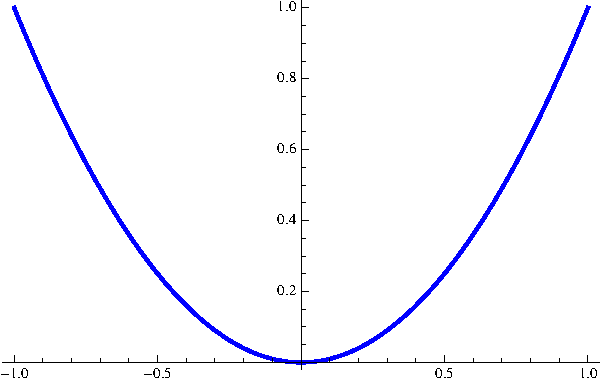
\includegraphics[width=0.5\textwidth]{plot}
\caption{A plot of a function.}
\label{fig:plot}
\end{figure}

\subsection{A subsection}

\lipsum[5]

\begin{align*}
1 + 1 + 1 &= 2 + 1 \\ &= 3.
\end{align*}

\subsubsection{A subsubsection}

\lipsum[17]

Here is a citation~\cite{greenwade93} with URL. Here is another
citation~\cite{MR4}, which is the earliest-numbered Math Review with a
functioning DOI: MR0000004. Finally, a reference to
equation~\eqref{eqn:eq1}. And a reference to Figure~\ref{fig:plot}.

\acknowledgements{\lipsum[20]}

%% if you use biblatex then this generates the bibliography
%% if you use some other method then remove this and do it your own way
\printbibliography



\end{document}
